% =====================================================================
% SOEN 6011 -- Deliverable 3, Problem 7
% Mind map: which user interface design principles apply
%
% Compile:  pdflatex mindmap.tex
% Produces a single landscape page suitable for the poster.
% =====================================================================

\documentclass[tikz,border=10pt]{standalone}

\usepackage{tikz}
\usetikzlibrary{mindmap,trees,shadows}

\begin{document}

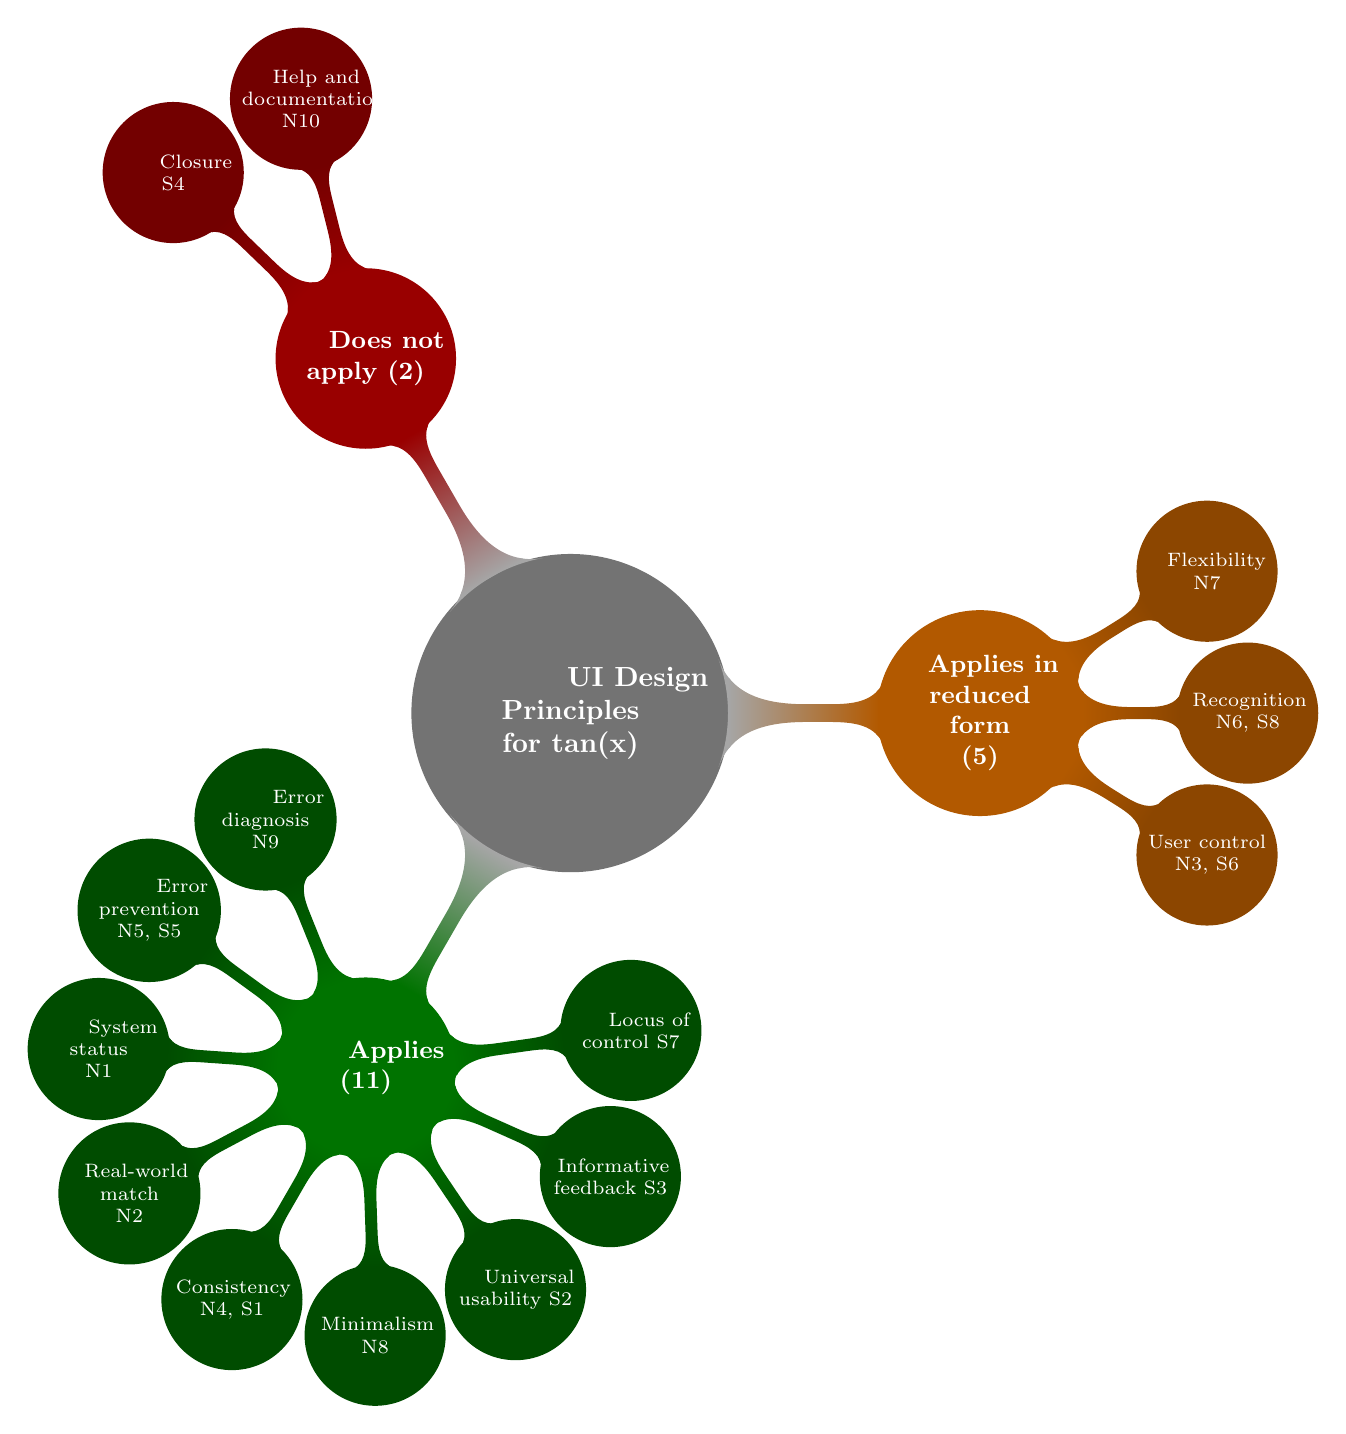
\begin{tikzpicture}[
    mindmap,
    grow cyclic,
    every node/.style={concept, execute at begin node=\hfil},
    concept color=black!35,
    text=black,
    level 1/.append style={level distance=5.2cm,
                           sibling angle=120,
                           font=\small\bfseries},
    level 2/.append style={level distance=3.4cm,
                           sibling angle=32,
                           font=\scriptsize},
]

\node [concept, concept color=black!55, text=white, font=\bfseries]
      {UI Design\\Principles\\for tan(x)}
  child [concept color=green!45!black, text=white] {
    node [font=\small\bfseries] {Applies\\(11)}
    child [concept color=green!30!black, text=white] {
        node {Error diagnosis\\N9} }
    child [concept color=green!30!black, text=white] {
        node {Error prevention\\N5, S5} }
    child [concept color=green!30!black, text=white] {
        node {System status\\N1} }
    child [concept color=green!30!black, text=white] {
        node {Real-world match\\N2} }
    child [concept color=green!30!black, text=white] {
        node {Consistency\\N4, S1} }
    child [concept color=green!30!black, text=white] {
        node {Minimalism\\N8} }
    child [concept color=green!30!black, text=white] {
        node {Universal\\usability S2} }
    child [concept color=green!30!black, text=white] {
        node {Informative\\feedback S3} }
    child [concept color=green!30!black, text=white] {
        node {Locus of\\control S7} }
  }
  child [concept color=orange!70!black, text=white] {
    node [font=\small\bfseries] {Applies in\\reduced form\\(5)}
    child [concept color=orange!55!black, text=white] {
        node {User control\\N3, S6} }
    child [concept color=orange!55!black, text=white] {
        node {Recognition\\N6, S8} }
    child [concept color=orange!55!black, text=white] {
        node {Flexibility\\N7} }
  }
  child [concept color=red!60!black, text=white] {
    node [font=\small\bfseries] {Does not\\apply (2)}
    child [concept color=red!45!black, text=white] {
        node {Help and\\documentation\\N10} }
    child [concept color=red!45!black, text=white] {
        node {Closure\\S4} }
  };

\end{tikzpicture}

\end{document}
